% Options for packages loaded elsewhere
\PassOptionsToPackage{unicode}{hyperref}
\PassOptionsToPackage{hyphens}{url}
%
\documentclass[
]{article}
\title{Sta 478 Project 1}
\author{Matthew Flanders}
\date{2/6/2022}

\usepackage{amsmath,amssymb}
\usepackage{lmodern}
\usepackage{iftex}
\ifPDFTeX
  \usepackage[T1]{fontenc}
  \usepackage[utf8]{inputenc}
  \usepackage{textcomp} % provide euro and other symbols
\else % if luatex or xetex
  \usepackage{unicode-math}
  \defaultfontfeatures{Scale=MatchLowercase}
  \defaultfontfeatures[\rmfamily]{Ligatures=TeX,Scale=1}
\fi
% Use upquote if available, for straight quotes in verbatim environments
\IfFileExists{upquote.sty}{\usepackage{upquote}}{}
\IfFileExists{microtype.sty}{% use microtype if available
  \usepackage[]{microtype}
  \UseMicrotypeSet[protrusion]{basicmath} % disable protrusion for tt fonts
}{}
\makeatletter
\@ifundefined{KOMAClassName}{% if non-KOMA class
  \IfFileExists{parskip.sty}{%
    \usepackage{parskip}
  }{% else
    \setlength{\parindent}{0pt}
    \setlength{\parskip}{6pt plus 2pt minus 1pt}}
}{% if KOMA class
  \KOMAoptions{parskip=half}}
\makeatother
\usepackage{xcolor}
\IfFileExists{xurl.sty}{\usepackage{xurl}}{} % add URL line breaks if available
\IfFileExists{bookmark.sty}{\usepackage{bookmark}}{\usepackage{hyperref}}
\hypersetup{
  pdftitle={Sta 478 Project 1},
  pdfauthor={Matthew Flanders},
  hidelinks,
  pdfcreator={LaTeX via pandoc}}
\urlstyle{same} % disable monospaced font for URLs
\usepackage[margin=1in]{geometry}
\usepackage{graphicx}
\makeatletter
\def\maxwidth{\ifdim\Gin@nat@width>\linewidth\linewidth\else\Gin@nat@width\fi}
\def\maxheight{\ifdim\Gin@nat@height>\textheight\textheight\else\Gin@nat@height\fi}
\makeatother
% Scale images if necessary, so that they will not overflow the page
% margins by default, and it is still possible to overwrite the defaults
% using explicit options in \includegraphics[width, height, ...]{}
\setkeys{Gin}{width=\maxwidth,height=\maxheight,keepaspectratio}
% Set default figure placement to htbp
\makeatletter
\def\fps@figure{htbp}
\makeatother
\setlength{\emergencystretch}{3em} % prevent overfull lines
\providecommand{\tightlist}{%
  \setlength{\itemsep}{0pt}\setlength{\parskip}{0pt}}
\setcounter{secnumdepth}{-\maxdimen} % remove section numbering
\usepackage{booktabs}
\usepackage{longtable}
\usepackage{array}
\usepackage{multirow}
\usepackage{wrapfig}
\usepackage{float}
\usepackage{colortbl}
\usepackage{pdflscape}
\usepackage{tabu}
\usepackage{threeparttable}
\usepackage{threeparttablex}
\usepackage[normalem]{ulem}
\usepackage{makecell}
\usepackage{xcolor}
\ifLuaTeX
  \usepackage{selnolig}  % disable illegal ligatures
\fi

\begin{document}
\maketitle

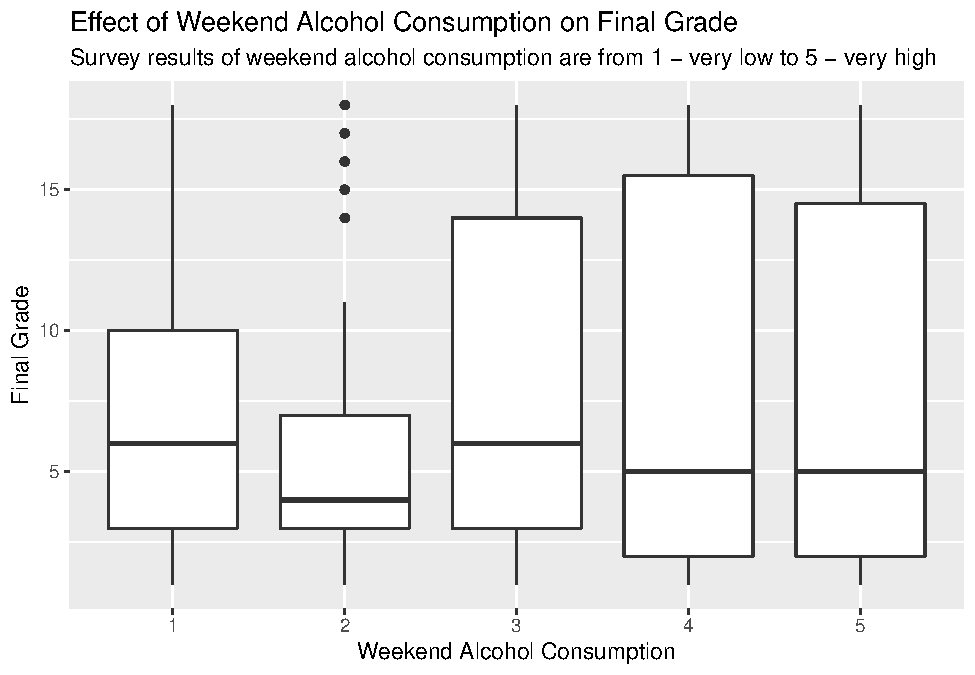
\includegraphics{proj.-1write-up_files/figure-latex/math-Walc-1.pdf}

\begin{table}

\caption{\label{tab:math-Walc}1-Way ANOVA Results(Final Grade ~ Weekend Alcohol Consumption)}
\centering
\begin{tabular}[t]{l|r|r|r|r|r}
\hline
  & Df & Sum Sq & Mean Sq & F value & Pr(>F)\\
\hline
Walc & 4 & 190.5869 & 47.64672 & 1.469466 & 0.2107179\\
\hline
Residuals & 390 & 12645.5650 & 32.42453 & NA & NA\\
\hline
\multicolumn{6}{l}{\rule{0pt}{1em}}\\
\end{tabular}
\end{table}
\newpage

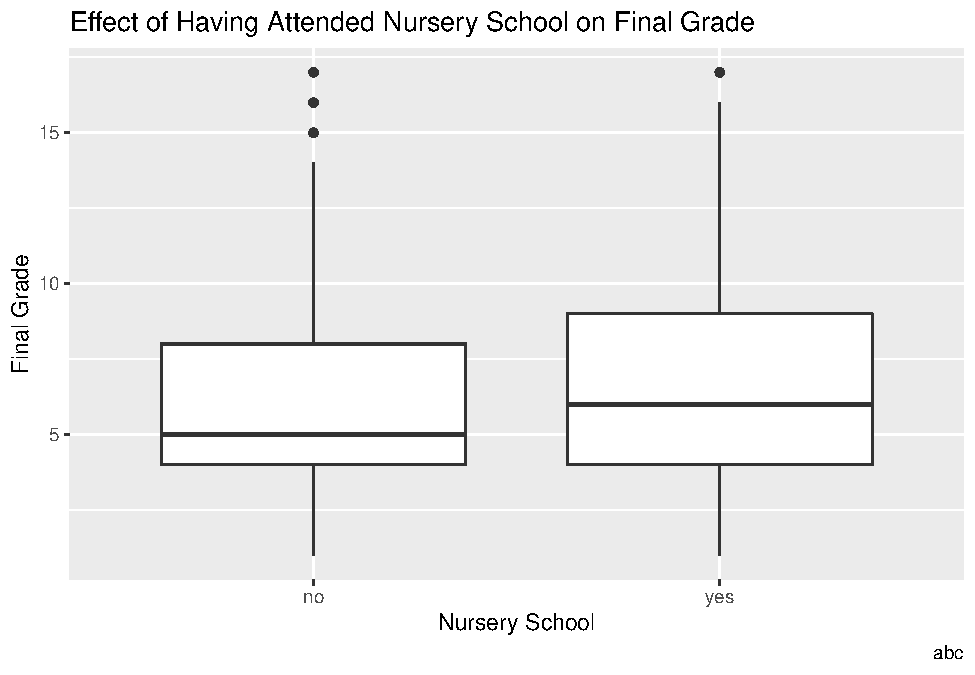
\includegraphics{proj.-1write-up_files/figure-latex/math-nursery-1.pdf}

\begin{tabular}{l|r|r|r|r|r}
\hline
  & Df & Sum Sq & Mean Sq & F value & Pr(>F)\\
\hline
nursery & 1 & 6.947937 & 6.947937 & 0.3972265 & 0.5287476\\
\hline
Residuals & 647 & 11316.756223 & 17.491122 & NA & NA\\
\hline
\end{tabular}
\newpage

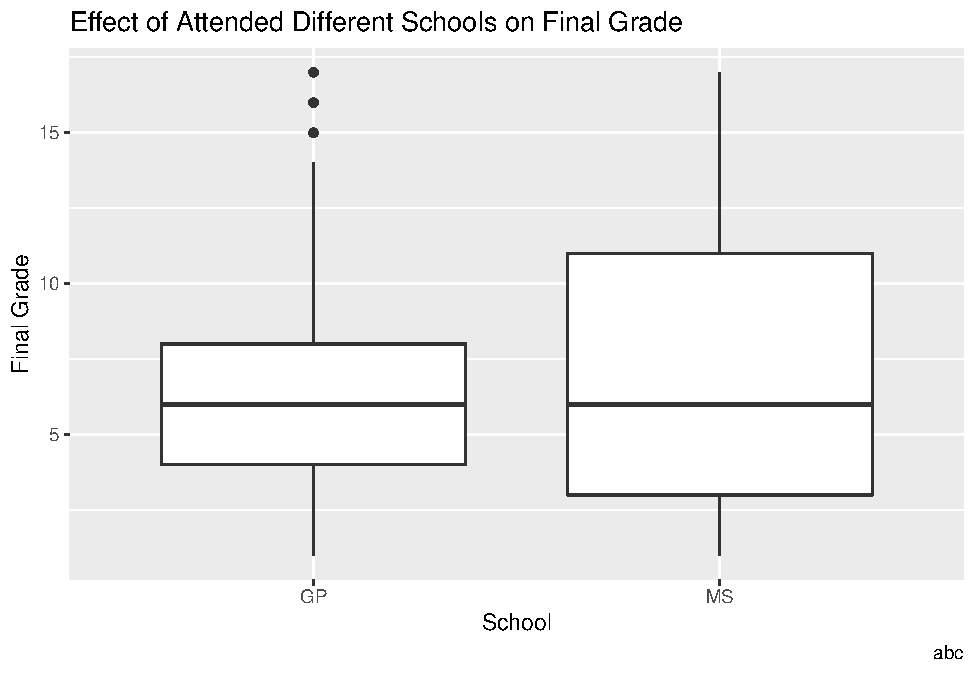
\includegraphics{proj.-1write-up_files/figure-latex/por-school-1.pdf}

\begin{tabular}{l|r|r|r|r|r}
\hline
  & Df & Sum Sq & Mean Sq & F value & Pr(>F)\\
\hline
school & 1 & 162.8945 & 162.89453 & 9.443111 & 0.0022085\\
\hline
Residuals & 647 & 11160.8096 & 17.25009 & NA & NA\\
\hline
\end{tabular}
\newpage

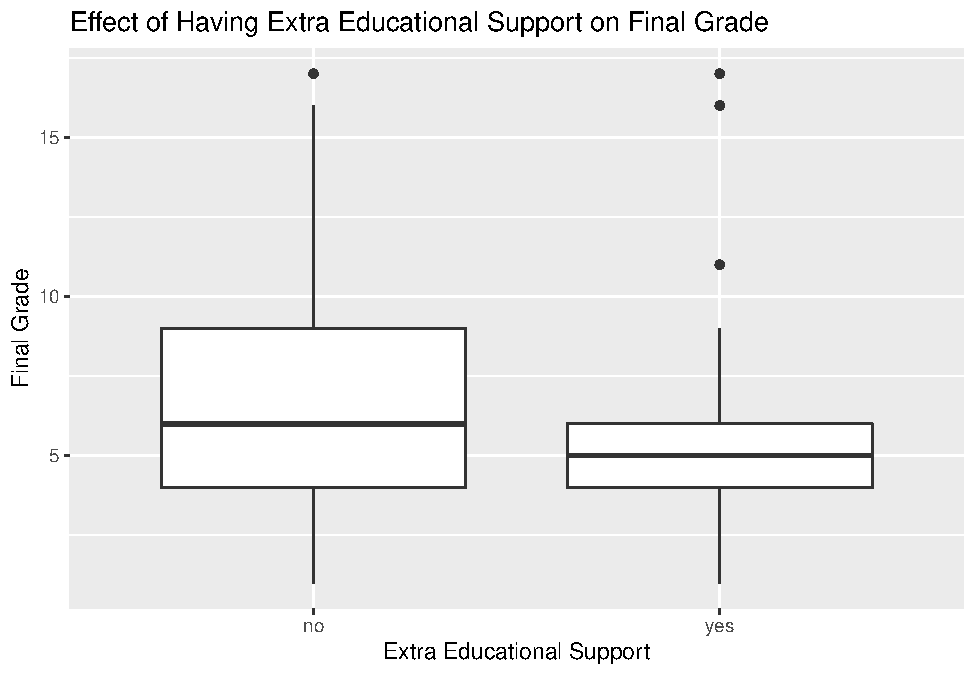
\includegraphics{proj.-1write-up_files/figure-latex/por-schoolsup-1.pdf}

\begin{tabular}{l|r|r|r|r|r}
\hline
  & Df & Sum Sq & Mean Sq & F value & Pr(>F)\\
\hline
schoolsup & 1 & 92.49711 & 92.49711 & 5.328513 & 0.0212937\\
\hline
Residuals & 647 & 11231.20705 & 17.35890 & NA & NA\\
\hline
\end{tabular}
\newpage

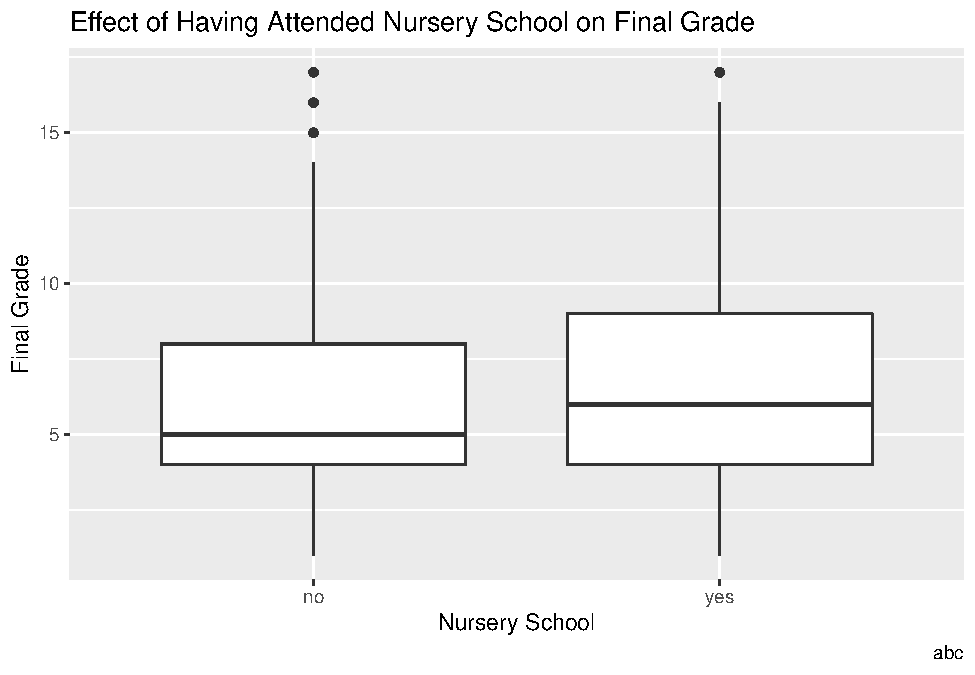
\includegraphics{proj.-1write-up_files/figure-latex/por-nursery-1.pdf}

\begin{tabular}{l|r|r|r|r|r}
\hline
  & Df & Sum Sq & Mean Sq & F value & Pr(>F)\\
\hline
nursery & 1 & 6.947937 & 6.947937 & 0.3972265 & 0.5287476\\
\hline
Residuals & 647 & 11316.756223 & 17.491122 & NA & NA\\
\hline
\end{tabular}

\end{document}
